\section{Trajectory Optimization}
\label{chapter:optimization}
It is important to state all the approximations and assumptions made for this problem.
\begin{itemize}
    \item The multi-rotor is approximated to a point
    \item The attitude is, at this point, ignored
    \item It can move in any direction
    \item It has limited acceleration
    \item It has limited speed
    \item The multi-rotor state $\sigma$ is defined by the position and speed of it's center of mass.
\end{itemize}

\subsection{Nomenclature}
It will be now introduced some nomenclature that will be used in this section. $\vec{\sigma}=[\sigma_0, ... , \sigma_{N-1}]$ is the vector with all the $N$ robot states along the trajectory, excluding the start and the goal states. $\sigma_s$ and $\sigma_g$ are the start and goal states respectively and these will not be subjected to optimization. Also $\sigma_i = [ \vec{p_i}, \vec{v_i}]$, where $\vec{p_i}$ and $\vec{v_i}$ corresponds to the position and speed vector of the robot in a given moment.  This means that $\sigma_i \in \mathbb{R}^4$ for a bi-dimensional environment  and $\sigma_i \in \mathbb{R}^6$ for three-dimensional environment (e.g. UAV). Let also $p_{i,j}$ represent the $j$th component of the robot position in the $i$th state and $v_{i,j}$ represent the $j$ component of the robot speed in the $i$th state. For example $p_{i,z}$  represents the $z$ component of the robot position in the $i$th state and $v_{i,y}$  the presents the $y$ component of the robot speed in the $i$th state.  Basically: $\sigma_i = [ \vec{p_i}, \vec{v_i}] = [p_{i,x}, p_{i,y}, p_{i,z}, v_{i,x}, v_{i,y}, v_{i,z}]$ (in 3 dimensional space).

It will be assumed that the robot acceleration $\vec{a}$ between two consecutive states is constant. Each state $\sigma_i$ represents the state of the robot at the time $t=t_s+(i+1)*\Delta t$ where $t_s$ is the start time. Therefore, the total trajectory time is given simply by $t_{total}= (N+1)* \Delta t$ (one time step from start to $\sigma_0$, N-1 time steps between the N states and one time step between $\sigma_{N-1}$ and the goal).

Considering this, the variables subjected to optimization will be $x=[\Delta t, \sigma_0, ..., \sigma_{N-1}]$. If it is written in the form of a vector of scalars (in 3 dimensional space):

$$x=[\Delta t, p_{0,x}, p_{0,y}, p_{0,z}, v_{0,x}, v_{0,y}, v_{0,z}, ... $$
$$..., p_{N-1,x}, p_{N-1,y}, p_{N-1,z}, v_{N-1,x}, v_{N-1,y}, v_{N-1,z}]$$

This will be the design variables of the problem, it is essential for the good comprehension of the following topics. The formulation of the optimization problem will be described in the following sections.

\subsection{Cost function}
The cost function chosen was a linear combination between the trajectory time $f_T(x)$ and energy consumption $ f_F(x)$. The scalar weights $k_T$ and $k_F$ allow to tune the relevance given to each of these costs. Such cost functions are suitable, for example, for minimizing the mission related costs. The cost function is then:

 \begin{equation}
     f(x)= k_T * f_T(x) + k_F * f_F(x)
     \label{eq:CostFunction}
 \end{equation}
 
 The time component is the total trajectory time, which is given as $(N+1)*\Delta t$ where $N$ represents the number of states subjected to optimization.
 
 To model the energy consumption for the multi-rotor it was used closed form expressions from the work by Marins et al. \cite{fuel}.  



\subsection{Kinematics}
The algorithm must respect the kinematics of the problem. It is assumed that the acceleration between to consecutive states $\sigma_i$ and $\sigma_{i+1}$ is constant. It is also assumed that the time elapsed for the robot to move from one state to another is $\Delta t$. With these assumptions, the position $\vec{p}_{i+1}$ should be given by:

\begin{equation}
    \vec{p}_{i+1}=\vec{p}_{i} + \frac{\vec{v}_{i+1}+ \vec{v}_{i+1} }{2}\Delta t
    \label{kinematics}
\end{equation}

To write Equation \ref{kinematics} in the form $c(x)=0$ the right side of Equation \ref{kinematics} is subtracted in both sides of the equation.
 
\subsection{Maximum speed and maximum acceleration}
The maximum speed constraint can be written as:

\begin{equation}
     |\vec{v}_i| < v_{MAX}
     \label{eq:maxSpeedRaw}
\end{equation}

Where $v_{MAX}$ is the maximum allowed speed. The maximum acceleration constraint can be intuitively stated as:

\begin{equation}
     |\vec{a_i}| < a_{MAX} \Leftrightarrow \frac{|\vec{v}_{i+1} - \vec{v}_{i}|}{\Delta t}  < a_{MAX}
     \label{eq:maxAccelraw}
\end{equation}
Where $a_{MAX}$ is the maximum allowed acceleration. To keep the derivatives simple, the form chosen for this inequity to be written was:

\begin{equation}
  |\vec{v}_{i+1} - \vec{v}_{i}| <  a_{MAX} \Delta t
  \label{eq:accelIneq}
\end{equation}{}

In order to create a constraint in the form $d(x)<0$ the right side of the inequality stated in Eq. \ref{eq:accelIneq} is subtracted to both sides of the inequation.

\subsection{Obstacle clearance}
\label{section:obstacleClearance}

It is now required to define the signed distance of a point to a convex obstacle. Let this signed distance $s(\mathcal{O}_k, \vec{p}_i)$ represent the distance from a point $\vec{p}_i$ to the closest point on the surface of a convex obstacle $\mathcal{O}_k$ , \emph{this distance is negative if the point $\vec{p}_i$ is inside the obstacle $\mathcal{O_K}$}.

The inequity that assures that the UAV is at least $d_{safe}$ away from any obstacle is
\begin{equation}
    s(\mathcal{O}_k, \vec{p}_i) > d_{safe}
\end{equation}

This formulation for the obstacle clearance constraints was formulated based on \cite{ref:SeqConvexOpt}. The signed distance is however, at the moment of writing, only available for spheres and cuboids in 3 dimensional environments and circles and rectangles in 2 dimensional environments. The algorithm also supports moving spheres (and circles). It can be expanded for general convex obstacles using, for example, the GJK and the expanding polytope algorithms \cite{GJK} \cite{EPA}. It is now necessary to limit the maximum time-step between waypoints to avoid the trajectory to "jumb over" obstacles, like it is shown in Figure \ref{fig:maxT}

\begin{figure}[H]
    \centering
    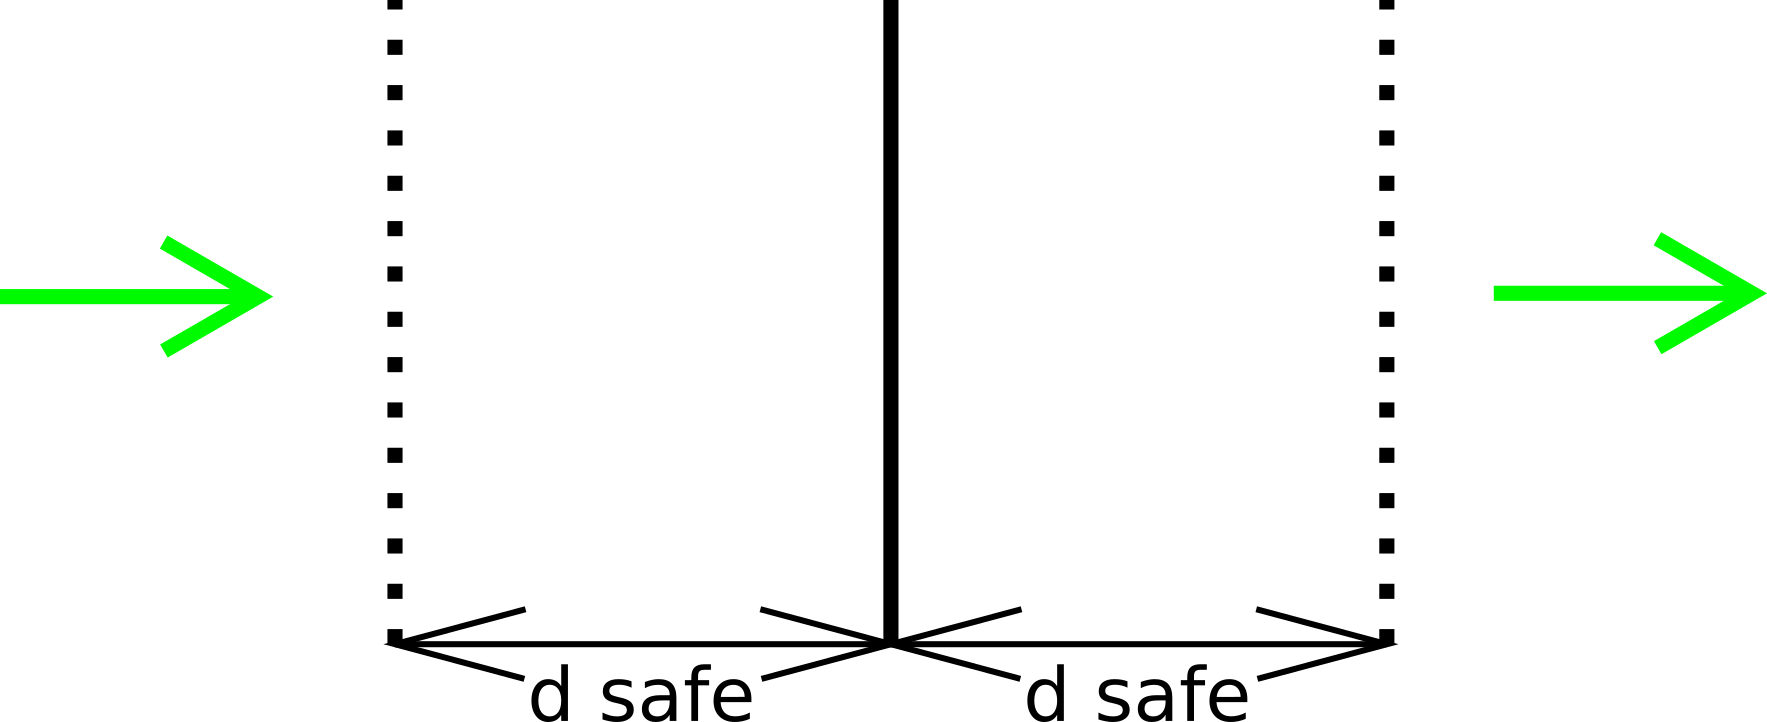
\includegraphics[width=0.8\linewidth]{Figures/05_optimization/maxT.png}
    \caption{Trajectory segment between two waypoints (green arrows) crosses an obstacle (black line) without any of the waypoints being closer than $d_{safe}$ to the obstacle.}
    \label{fig:maxT}
\end{figure}

\par
To enable the usage of bigger trajectory segments, which reduce the number of way-points and increases the algorithm performance, new constraints were imposed. These new constraints assure that a number of intermediate points (equally spaced points in each trajectory segment between way-points) are not in collision with any obstacle. 
\par
To validate the performance improvement, the algorithms were used to optimize a trajectory from a first iteration (shown in Figure \ref{fig:x0}) to a local minima. This optimization was repeated replacing $M-1$ out of $M$ waypoints by intermediate collision checking points, as shown in Fig. \ref{fig:interClean}. 

\begin{figure}[H]
    \centering
    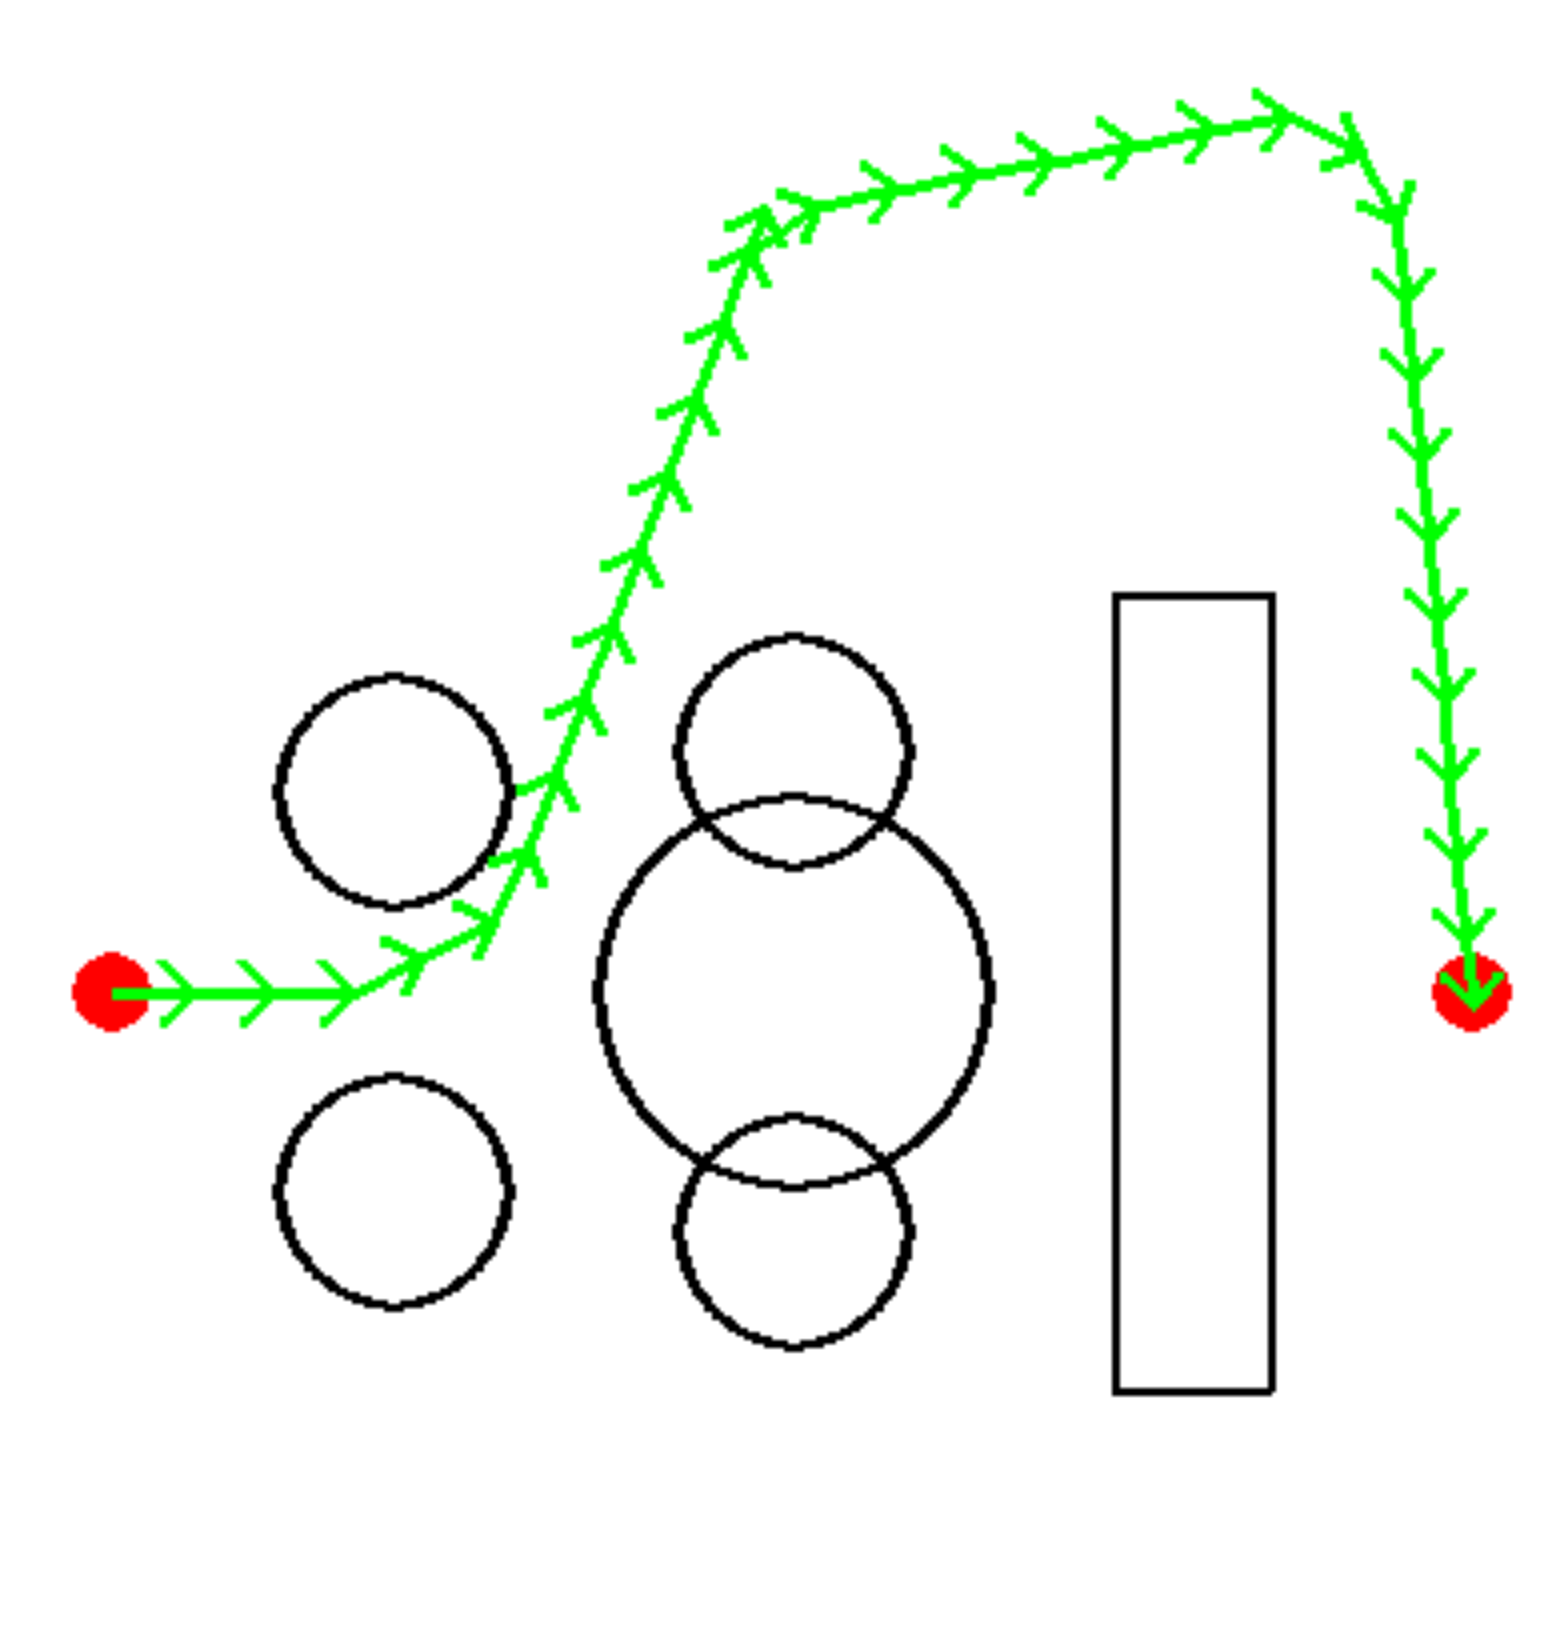
\includegraphics[width=0.6\linewidth]{Figures/05_optimization/initialIter.png}
    \caption{Initial trajectory, to be optimized}
    \label{fig:x0}
\end{figure} 

\begin{figure}[H]
    \centering
    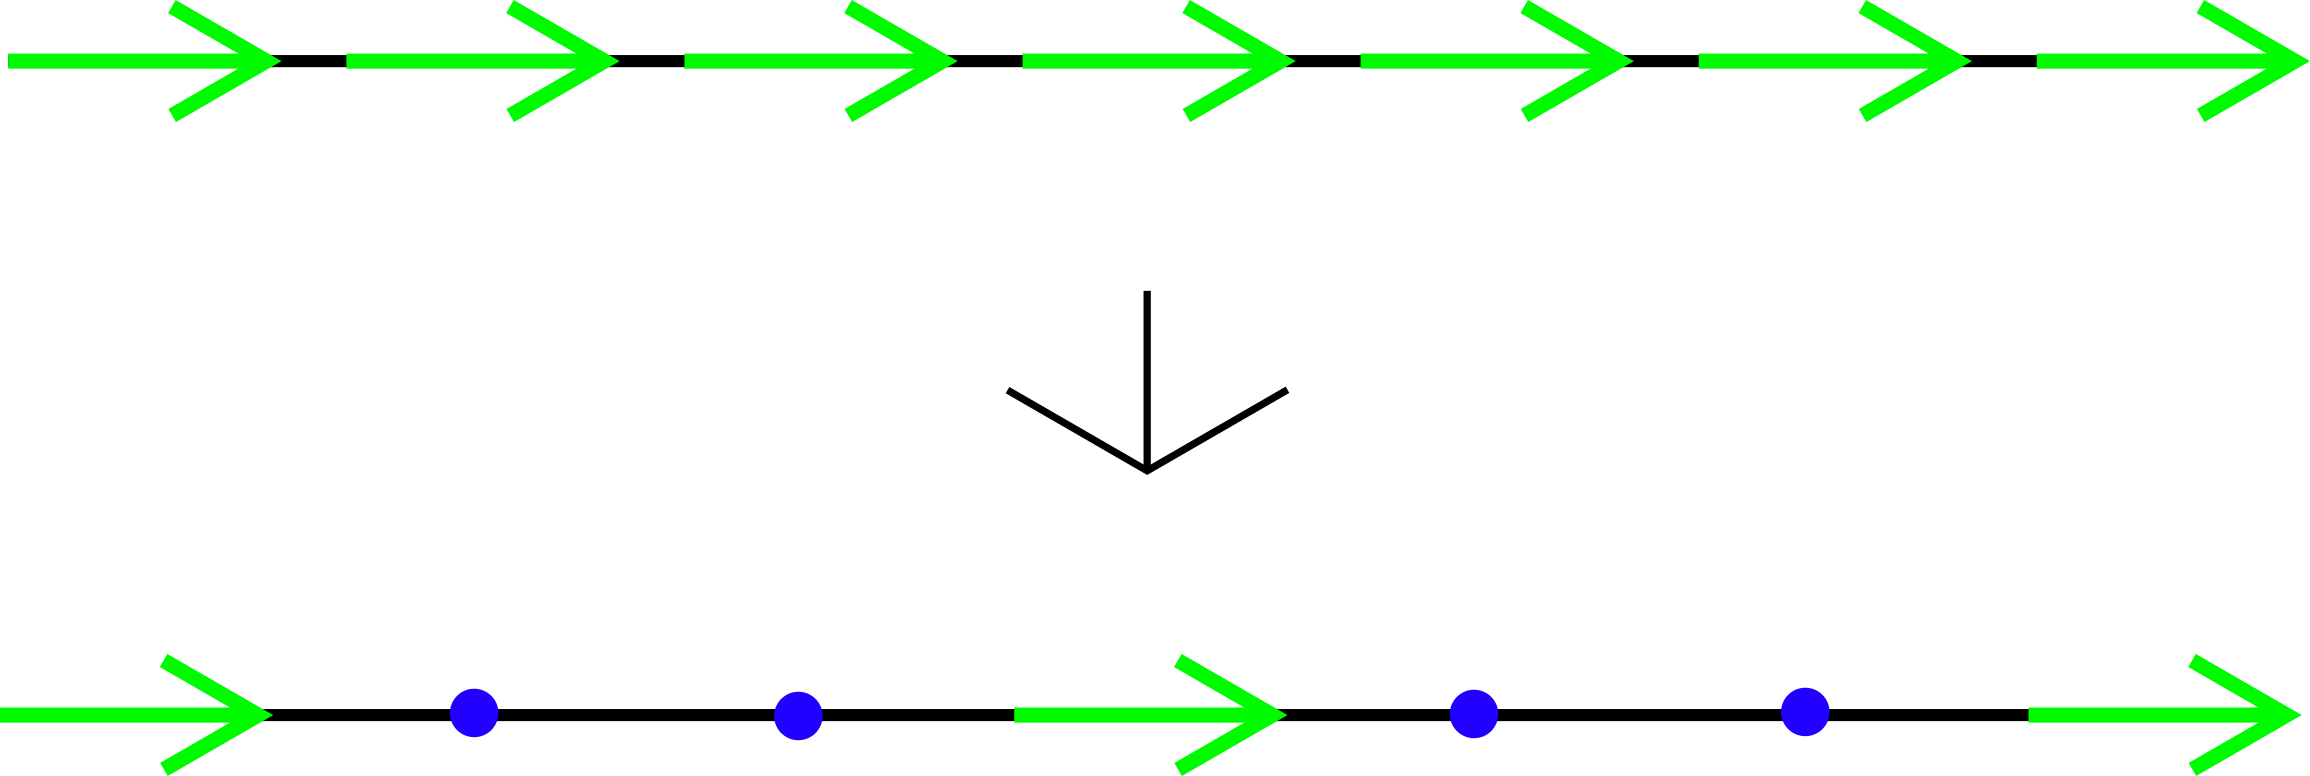
\includegraphics[width=0.8\linewidth]{Figures/05_optimization/cleanInter.png}
    \caption{Trajectory before (top) and after (bottom) exchanging waypoints (green arrows) for intermediate collision checking points (blue  circles). In this illustration the number of intermediate points per trajectory segment chosen was 2 ($M$=3).}
    \label{fig:interClean}
\end{figure}

\par
After multiple simulations it is possible to observe that the computational time is smaller if some way-points are replaced for these intermediate collision checking points. The computational time, however, increases if the number of replacements is further increased. These results are shown in Table \ref{IPOPTresultsInter2}.

\begin{table}[H]
    \centering
    \begin{tabular}{c|l|l}
        $M-1$ & mean ($s$) & variance ($s^2$) \\ \hline
        0 & 0.91429 & 0.00141 \\
        1 & 0.70004 & 0.00007 \\
        2 & 0.44371 & 0.00046 \\
        3 & 0.50951 & 0.00020 \\
        5 & 0.85712 & 0.00011 \\ \hline
    \end{tabular}
    \caption{Computational time until local-minima is reached, for different numbers of intermediate points per trajectory segment $M-1$, using 10 runs for each. }
    \label{IPOPTresultsInter2}
\end{table}


\subsection{Problem formulation}
\label{section:formulations}

The problem formulation can finally be stated in a simplified intuitive way:

\begin{equation}
    \begin{matrix*}[l]
    min && k_T * f_T(x) + k_F * f_F(x)  \\
    s.t.&& \vec{p}_{i+1}=\vec{p}_{i} + \frac{\vec{v}_{i+1}+ \vec{v}_{i+1} }{2}\Delta t\\
        && |\vec{v_i}| < v_{MAX}\\
        && |\vec{v}_{i+1}-\vec{v_i}| < a_{MAX} \Delta t\\
        && s(\mathcal{O}_k, \vec{p}_i) >  d_{safe}\\
        && s(\mathcal{O}_k, \vec{p}_{inter (i,m)} ) >  d_{safe}\\
    \end{matrix*}
    \label{formulation2}
\end{equation}

In Equation \ref{formulation2} $\vec{p}_{inter (i,m)}$ represents the $m$th intermediate collision checking point for the trajectory segment that joins two consecutive way-points ($\sigma_i$ to $\sigma_{i+1}$). $s(\mathcal{O}_k, \vec{p}_i) $ represents the signed distance between a point a point $\vec{p}_i$ and an obstacle $\mathcal{O}_k$.
